%\documentclass[english,twoside]{article}
\documentclass[english,twoside]{labmanual} 
%labmanual.cls is a modified version of article.cls, tweaked to handle \part{} differently

%% LyX 1.1 created some parts of this file.  For more info, see http://www.lyx.org/.
%% Do not edit unless you really know what you are doing.

\usepackage[T1]{fontenc}
\usepackage[nomarginpar]{geometry}
\usepackage{tocloft} %Allow us to leave page numbers for Parts out of table of contents
\cftpagenumbersoff{part} %No page numbers for Parts out of table of contents
\renewcommand{\cftsecdotsep}{\cftsubsecdotsep}
%\usepackage{newclude} %Allows use of /include*{}
%DANGER DANGER: newclude is NOT compatible with package xr, used for external references.
\geometry{verbose,letterpaper}
\usepackage{fancyhdr}
\usepackage{babel}
\setlength\parskip{\medskipamount}
\setlength\parindent{0pt}
\usepackage{graphicx}
\usepackage{wrapfig}
%\usepackage{epstopdf} %this package apparently allows pdflatex to work on this document, since all we use are eps figures.
\usepackage{comment}
\usepackage{esvect}
\usepackage{amsmath} %uncommented by MT 5/2015, used in "E near charged rod"
\usepackage{mathtools} %added by MT 6/2015, for access to dcases environment in finding_v_from_e
\usepackage{tabularx} %added by MT 6/2015, for fixed width columns, used in rc_circuits
\usepackage{microtype}
\usepackage{titlesec}
\usepackage{xr}

%For fixed width columns:
\newcolumntype{L}[1]{>{\raggedright\arraybackslash}p{#1}}
\newcolumntype{C}[1]{>{\centering\arraybackslash}p{#1}}
\newcolumntype{R}[1]{>{\raggedleft\arraybackslash}p{#1}}


\addtolength{\oddsidemargin}{1.0cm} %without these two lines, larger margin is on the OUTSIDE.  We want the larger edge on the INSIDE, to allow room for the three hole punches
\addtolength{\evensidemargin}{-1.0cm}

\setlength\topmargin{0.2in}
\addtolength{\hoffset}{-1.0cm}
\addtolength{\textwidth}{2.0cm}
\addtolength{\voffset}{-1.5cm} %This line is apparently needed on some versions of MikTex XeLatex.  Comment out if your pages appear shifted too high.
\addtolength{\textheight}{3.5cm}
% define a strut for extra vertical space in tables.
\newcommand{\hi}{\rule[-2mm]{0mm}{6mm}}

\pagestyle{fancy}
%\fancyhead[LE,RO]{\slshape \rightmark} %This is the default for fancy page style
%\fancyhead[LO,RE]{\slshape \leftmark}
\fancyhead[LO,RE]{\slshape \rightmark} 
\fancyhead[LE,RO]{\slshape \leftmark} % Reversed LE, RO to  LO,RE to make headers come out correctly on even/odd pages



%%%%%%%%%%%%%%%%%%%%%%%%%%%%%% LyX specific LaTeX commands.
\providecommand{\LyX}{L\kern-.1667em\lower.25em\hbox{Y}\kern-.125emX\@}
\newenvironment{LyXParagraphIndent}[1]%
{
  \begin{list}{}{%
    \setlength\topsep{0pt}%
    \addtolength{\leftmargin}{#1}
    \setlength\parsep{0pt plus 1pt}%
  }
  \item[]
}
{\end{list}}
%% Special footnote code from the package 'stblftnt.sty'
%% Author: Robin Fairbairns -- Last revised Dec 13 1996
\makeatletter
\let\SF@@footnote\footnote
\def\footnote{\ifx\protect\@typeset@protect
    \expandafter\SF@@footnote
  \else
    \expandafter\SF@gobble@opt
  \fi
}
\expandafter\def\csname SF@gobble@opt \endcsname{\@ifnextchar[%]
  \SF@gobble@twobracket
  \@gobble
}
\edef\SF@gobble@opt{\noexpand\protect
  \expandafter\noexpand\csname SF@gobble@opt \endcsname}
\def\SF@gobble@twobracket[#1]#2{}
\makeatother


%I make use of some latex features to manage the section numbers. To use those you have to insert the following lines into the latex preamble (before the %"\begin{document}" command).

% two new commands to do labelling. - gpg 12/4/13
\newcommand{\customlabel}[2]{%
\protected@write \@auxout {}{\string \newlabel {#1}{{#2}{}}}}

\newcommand{\actlabel}[1]{%
\protected@write \@auxout {}{\string \newlabel {#1}{{\arabic{activity}}{}}}}

\newcommand{\makelabheader}
%{Name: \rule{2.0in}{0.1pt}\hfill{}Section: \rule{1.0in}{0.1pt}\hfill{}Date: \rule{1.0in}{0.1pt}}
{Name: \rule{2.0in}{0.1pt}\hfill{}Lab Partner(s): \rule{3.0in}{0.1pt}}

%\newcommand{\dir131}{../../131/StudentGuideModule1} %This does not work, because commands can only be made of numeric characters, not numbers.

%A new command for putting a box around a paragraph:
\newenvironment{newboxed} %maybe there's a better way to do this.  I just cribbed from the web. --MT
    {\begin{center}
    \begin{tabular}{|p{0.9\textwidth}|}
    \hline\\
    }
    { 
    \\\\\hline
    \end{tabular} 
    \end{center}
    }

\newcounter{activity}

%  The following command, \answerspace, should be used to replace \vspace.
%  \vspace{} is not ideal for an answer space for students, for two reasons:
%  1. It can be ignored if it comes at the end of a page, and
%  2. The spacing is exact, and Latex will not stretch or compress it at all to make things fit on a page, which means
%  that other things WILL get stretched or compressed to make things fit, which means those other things will 
%  end up looking bad, and leading to a lot of underfull \vbox warnings.
%  \answerspace fixes both of those problems, specifically allowing the space to grow to up to twice the stated size.
\newcommand{\answerspace}[1]{\vspace*{#1 plus #1}}

%  The next several lines implement \includelab, which replaces \include.
%  Usage is \includelab{1}{file} to include it, or \includelab{0}{file} to NOT include it.  
%  But all 0's can be overridden by writing \includealllabstrue in the master.tex file, which is easier than deleting 
%  fifty individual `%' signs and then remembering to put them all back, which is what you had to do before.
%  \includeonly still works as you expect it to.
\newif\ifincludealllabs
\newcommand{\includelab}[2]{
	\ifnum#1=1
		\include{#2}
	\else {
		\ifincludealllabs
		 	\include{#2}
		\fi}
	\fi
}
 %all general latex packages, commands, and definitions now here.
\externaldocument{master}

%syntax: \includeonly{lab1,lab2,lab3} with no spaces after the commas.
%\includeonly{biot_savart_law/biot_savart_law, charge_density/charge_density,eoverm/eoverm }
%DANGER: The includeonly statement will make a document that does NOT have sequential page numbers.

\newcommand{\supplementmark}{CB}

\titleformat{\section}{\normalfont\Large\bfseries}{\supplementmark \thesection}{1em}{}
\fancyhead[LO,RE]{\slshape \rightmark} 
\fancyhead[LE,RO]{\slshape \supplementmark \leftmark} % Reversed LE, RO to  LO,RE to make headers come out correctly on even/odd 

\begin{document}

\setcounter{page}{157}  %Set this to desired first page
\setcounter{section}{37} %set this to desired first section number MINUS ONE

%--------------------------------------------
%Put include statements for labs below here.

\section{Electrostatics}

\makelabheader %(Space for student name, etc., defined in master.tex)

\textbf{Objective}

\begin{itemize}
\item To understand the basic phenomena of electric charges at rest.
\end{itemize}
\textbf{Introduction}

Atoms consist of a central nucleus made up of protons and neutrons
surrounded by one or more electrons. While the nuclei of solids are
essentially localized, some of the electrons may be free to move about.
A substance which has as many electrons as it has protons is said
to be electrically neutral. Dissimilar objects have different affinities
for electrons. When two such objects, initially neutral, are rubbed
together, the friction may cause electrons to pass from one to the
other. After separation, neither object is neutral. Each is said to
have been {}``charged by friction''. An isolated, electrified object
becomes neutral again if its electron-proton balance is restored.
A convenient means for accomplishing this is to connect the object
to earth by means of a conductor, through which electrons readily
travel. This process is called {}``grounding the body''. Since an
electrified object is referred to as {}``charged'', grounding is
also referred to as {}``discharging''.

Substances through which electrons do not move easily are called {}``non-conductors'',
or {}``insulators''. Experiment has shown that when rubber and wool
are rubbed together, electrons pass form the wool to the rubber. The
electrons remain on the surface of the rubber--a non-conductor--where
they were transferred.

Rubbing a metal rod with a wool cloth can also transfer electrons.
This rod, however, is a conductor and electrons pass through it to
the experimenter and then to the earth. People, made mostly of salt
water, are good conductors, as well. Metal that is isolated, however,
can be electrified. This can be demonstrated with an electroscope,
which has a metal knob connected to a stem from which a thin metal
leaf hangs. An insulator prevents contact of these metal parts with
the case, and consequently the earth.

\textbf{Apparatus}

\begin{itemize}
\item electroscope
\item rubber and glass rods
\item wool and silk cloth
\item plastic rod with metal disc mounted on one end
\end{itemize}
\textbf{Activity 1: Charging by Friction}

\begin{enumerate}
\item Be sure the electroscope is discharged by touching the knob with your
finger. Explain what happened and why you are convinced the electroscope
is discharged.\vspace{15mm}

\item \textbf{Prediction:} If you rub the knob of an electroscope with a
wool cloth, what will be the state of the electroscope when you remove
the cloth? Explain.\vspace{15mm}

\item Gently and repeatedly rub the knob of the electroscope with the wool cloth for a couple of minutes. Remove the cloth. Note any differences in the electroscope from its appearance before you rubbed.\vspace{15mm}

\item Explain what, if anything, happened.\vspace{15mm}

\end{enumerate}
\textbf{Activity 2: Charging by Contact}

\begin{enumerate}
\item Discharge the electroscope as before.
\item Charge the disc at the end of the plastic rod by friction with
the wool cloth.
\item Does anything occur in the electroscope when you bring the disc close
to the knob without touching it?\vspace{15mm}

\item \textbf{Prediction:} What will happen to the electroscope if you repeatedly
touch its knob with a freshly charged object?\vspace{15mm}

\item Touch the disc to the knob; rub the disc again and again touch it
to the knob; repeat this procedure two or three more times. Describe
any changes to the electroscope.\vspace{15mm}

\item Repeat the procedure above until the electroscope's leaf is at approximately
a twenty degree angle with the stem.
\end{enumerate}
\textbf{Activity 3: Kinds of Electrification}

\begin{enumerate}
\item Electrify one end of the rubber rod by wrapping the wool cloth around
the rod, squeezing the wool against the rod, twisting the rod vigorously
to ensure good contact, and separating the wool from the rod.
\item \textbf{Prediction:} What will happen when you bring the electrified
end of the rubber rod toward, but not touching, the electroscope's
knob? What will happen if you do the same with the wool cloth?\vspace{15mm}

\item Bring the charged end of the rubber rod toward the knob, but do not
touch it. Record what happens.\vspace{15mm}

\item Repeat number 3 with the wool cloth.\vspace{15mm}

\item What differences were there between the trial with the rod and the
trial with the cloth?\vspace{15mm}

\item How would you account for these differences?\vspace{15mm}

\item \textbf{Note:} By definition, the electrical state of the rubber after
being rubbed by the wool is negative. That is, an object that has
an excess of electrons is said to be negatively charged. Realize that
this is only a convention.
\item If the rubber is said to be negatively charged, in what electrical
state is the wool cloth?\vspace{15mm}

\item How can an electroscope be used to determine the nature of any charge?\vspace{15mm}

\item Rub the end of the glass rod with the silk cloth and determine the
charge of each (positive or negative) after they are separated.\vspace{15mm}

\end{enumerate}
\textbf{Activity 4: Action of the Electroscope}

\begin{enumerate}
\item \textbf{Discussion:} Two facts explain the rise or fall of the leaves
of an electroscope: (a) Like charges repel (unlike charges attract);
and (b) Free electrons move about in a conductor when an electric
force acts upon them.
%\item Discharge the electroscope.
%\item \textbf{Prediction:} What will happen when you bring the charged rubber
%rod near the discharged electroscope? What will happen if you do the
%same with the wool cloth?\vspace{15mm}

%\item Test your predictions; record the results; try to explain them.\vspace{15mm}

%\item Do the leaf and stem now become positive or negative?\vspace{15mm}

\item In Activity 3, the electroscope was negatively charged before either
the rubber rod or the wool cloth was brought toward the knob. When the rubber 
rod approaches the knob (in Acticity 3 number 3), in which direction do the 
free electrons in the electroscope move (up toward the knob or down toward the 
leaf)? Does the electron displacement increase or decrease the electrostatic
force separating the leaf from the stem?\vspace{15mm}

\item When the wool cloth approaches the knob (in Activity 3 number 4), which 
way do the free electrons move?

\end{enumerate}

\newpage

\textbf{Activity 5: Charging by Induction}

\begin{enumerate}
\item Discharge the electroscope.
\item \textbf{Prediction:} What will be the effect on the electroscope if
you perform the following experiment: while grounding the electroscope
with your finger, bring an electrified rubber rod near the knob, then
take away your finger and then the rod (in that order)?\vspace{15mm}

\item Carry out the experiment and describe the result.\vspace{15mm}

\item Explain the result and why your prediction agreed or disagreed with
it.\vspace{15mm}

\item \textbf{Prediction:} Note that no electrons moved between the rod
and the electroscope. What charge has been induced on the electroscope?\vspace{15mm}

\item Test your prediction with the negatively charged rubber rod and the
positively charged wool.
\item Does the test verify or contradict your prediction?\vspace{15mm}
\end{enumerate}



\section{Ohm's Law}

\makelabheader %(Space for student name, etc., defined in master.tex)

\textbf{Objectives}

\begin{itemize}
\item To investigate the most important principle in electronics.
\item To determine how resistors in series and parallel add.
\end{itemize}
\textbf{Introduction}

The rate at which electric charge flows through a conductor is called
the electric current. In order to have a current, a potential difference,
or voltage is necessary. We first want to determine the relationship
between the potential difference at two ends of a conductor and the
current flowing through it.

\textbf{Note}: Do not turn on a power supply until you are sure your
circuit is correct. If you are at all unsure, please ask your instructor
to approve your setup. Ammeters can be instantly and permanently ruined
by an improper connection. Be sure to turn off the power supply before
making any changes to the circuit.

\textbf{Apparatus}

\begin{itemize}
\item Power supply
\item Two resistors
\item Leads and alligator clips
\item DC Milliammeter
\item Multimeter
\end{itemize}
\textbf{Activity 1: Ohm's Law}

\begin{itemize}
%\item Connect two rheostats (or variable resistors) in series as shown in
%the figure below. Set R\( _{1} \) at about the halfway point and
%R\( _{2} \) at the maximum. Connect an ammeter as shown. Also, connect
%a voltmeter across (that is, connect a probe to each side of) R\( _{1} \).
%\item The fixed resistor will be considered an ``unknown'' and will be called 
%R\( _{1} \). The variable resistor will be called R\( _{2} \), and will be used 
%to vary the current. Connect the two resistors in series as shown in the 
%figure. Set R\( _{2} \) at its maximum value. Connect a milliammeter as shown, 
%at the point marked ``A'' (for ``ammeter''). Leave the positive lead to the 
%power supply disconnected.
\item With the power supply off, turn the coarse current control all the way up 
and both voltage controls all the way down.  Connect one of the resistors in 
series with the milliammeter (marked ``A'' for ``ammeter'') as shown in the 
figure below. Be sure the polarity of the milliammeter is as shown.
\end{itemize}
\vspace{0.3cm}
{\centering \resizebox*{0.35\textwidth}{!}{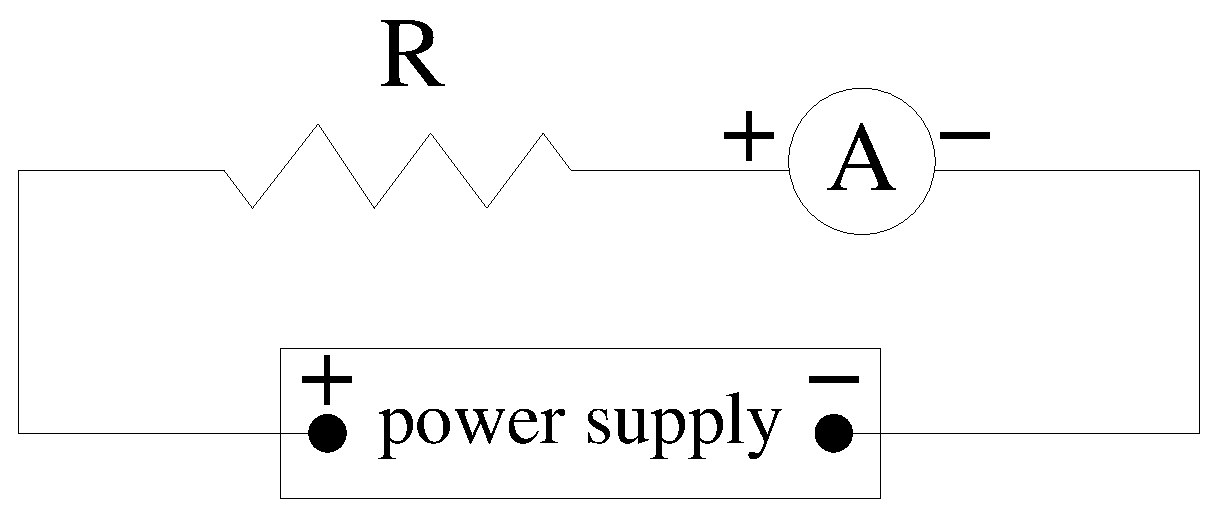
\includegraphics{ohms_law/ohms_law_fig_3.eps}} \par}
\vspace{0.3cm}

\begin{itemize}
\item When sure of your circuit, turn on the power supply, and turn the coarse 
voltage control up until the milliammeter reads 20 ma. Measure the voltage 
across the resistor (with the multimeter set for DC voltage) and record both voltage and current here. Include an uncertainty in the voltage measurement.
\vspace{10mm}

%\item Reduce the resistance of R\( _{2} \) and record the current and voltage
%three more times by turning down R\( _{2} \) in approximately equal steps so 
%that for the last time R\( _{2} \) is turned completely down. 
%Record your results here:\vspace{30mm}

\item Now turn the coarse voltage control up and record current and voltage 
for four more values of current: 40, 60, 80, and 100 ma. Include uncertainties
 in the voltage measurements.
\vspace{30mm}

\item Turn off the power supply.

\item Using $Excel$, plot your five pairs of readings with the voltage on the 
vertical axis and the current on the horizontal axis. Include the origin as a 
sixth point (why is this valid?).
\vspace{6mm}
\item Fit a straight line to the points (including the origin).
Include a trendline with equation.
\item Use the LINEST function in $Excel$ (see \textbf{Appendix C}) to 
determine the slope of the line and its uncertainty.  What is the meaning 
of the slope? Write its value with uncertainty here (including units):
\vspace{20mm}

\item Print the graph and include it with this unit.

\item Remove the resistor from the rest of the circuit and use the ohmmeter
option on the multimeter to measure the resistance of R directly.
Does it fall within the range of values determined above? Can you think of 
a reason for any discrepancy?
\vspace{20mm}

\item What is the general relationship between voltage, current, and resistance?
This is Ohm's Law.\vspace{15mm}

\item Why is the origin a legitimate point on the curve?\vspace{15mm}

\end{itemize}
\textbf{Activity 2: Resistors in Series}

\begin{itemize}
%\item Turn rheostat R\( _{2} \) to its maximum setting. Connect the multimeter
%across this resistor, being sure to set it for reading voltages.
%\item When you are sure the circuit is set, turn on the power supply and
%record the current and voltage. Turn off the power supply.\vspace{10mm}

%\item \textbf{Prediction}: Based on your measurements, predict the resistance
%of R\( _{2} \).\vspace{15mm}

%\item Remove and measure the resistance of R\( _{2} \). Record the percent
%difference between your prediction and measurement. Replace R\( _{2} \).\vspace{30mm}

%\item Was the current this time different from the first reading in Activity
%1?\vspace{15mm}

\item Turn the voltage control down to zero, and connect two resistors in 
series as shown in the figure below.
\end{itemize}
\vspace{0.3cm}
{\centering \resizebox*{0.35\textwidth}{!}{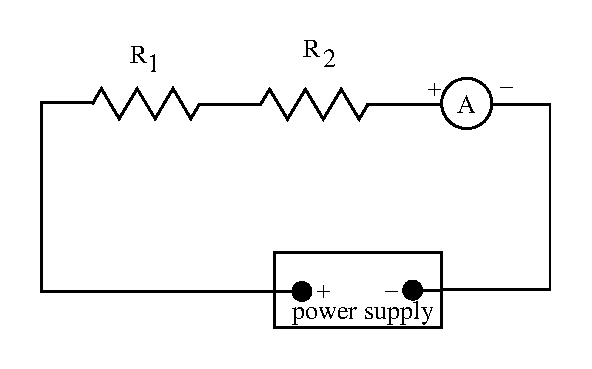
\includegraphics{ohms_law/ohms_law_fig_1.eps}} \par}
\vspace{0.3cm}

\begin{itemize}

\item Turn on the power supply and turn up the coarse voltage control to 
approximately 10 volts. Measure the voltages across R\( _{1} \), R\( _{2} \), 
and the milliammeter. (The voltage across the milliammeter may be in \underline{millivolts}.) Also measure the total voltage across all three elements 
in series. Include uncertainties in each measurement. Record your results here:
\vspace{20mm}

\item How is the last measurement related to the three individual 
measurements?
\vspace{10mm}

\item What can you conclude about the voltage across resistors in series?
\vspace{10mm}

\item Measure the current in the series circuit and record it here:
\vspace{10mm}

\item Using Ohm's Law, determine the total resistance of the circuit from the 
total voltage and the current which you have measured.
\vspace{10mm}

%\item Connect the multimeter across both resistors, being sure to switch
%to voltage readout.
%\item When you are sure the circuit is correct, turn on the power supply
%and record the current and voltage. Turn off the power supply.\vspace{10mm}

%\item Has the current changed?\vspace{15mm}

%\item Has your previous conclusion been substantiated or refuted?\vspace{15mm}

%\item How is the voltage just measured related to the first voltage measurements
%in Activities 1 and 2?\vspace{15mm}

%\item What can you conclude about the voltage across resistors in series?\vspace{15mm}

\item Turn the voltage control down to zero and turn off the power supply.

\item Calculate R\( _{1} \), R\( _{2} \), and R\( _{A} \) from Ohm's Law and 
your above readings. From these three values, determine the total resistance of 
the circuit. Does it agree with the value you calculated above? Record your 
results here:
\vspace{20mm}

\item What can you conclude about the total resistance in a circuit 
containing resistors in series?\vspace{15mm}

\end{itemize}

\pagebreak

\textbf{Activity 3: Resistors in Parallel}

\begin{itemize}
\item Connect the two resistors in parallel as shown in figure \textbf{a} 
below, with the milliammeter at the point marked ``A''. Have circuit checked 
before continuing.
\end{itemize}
\vspace{0.3cm}
\begin{center}
%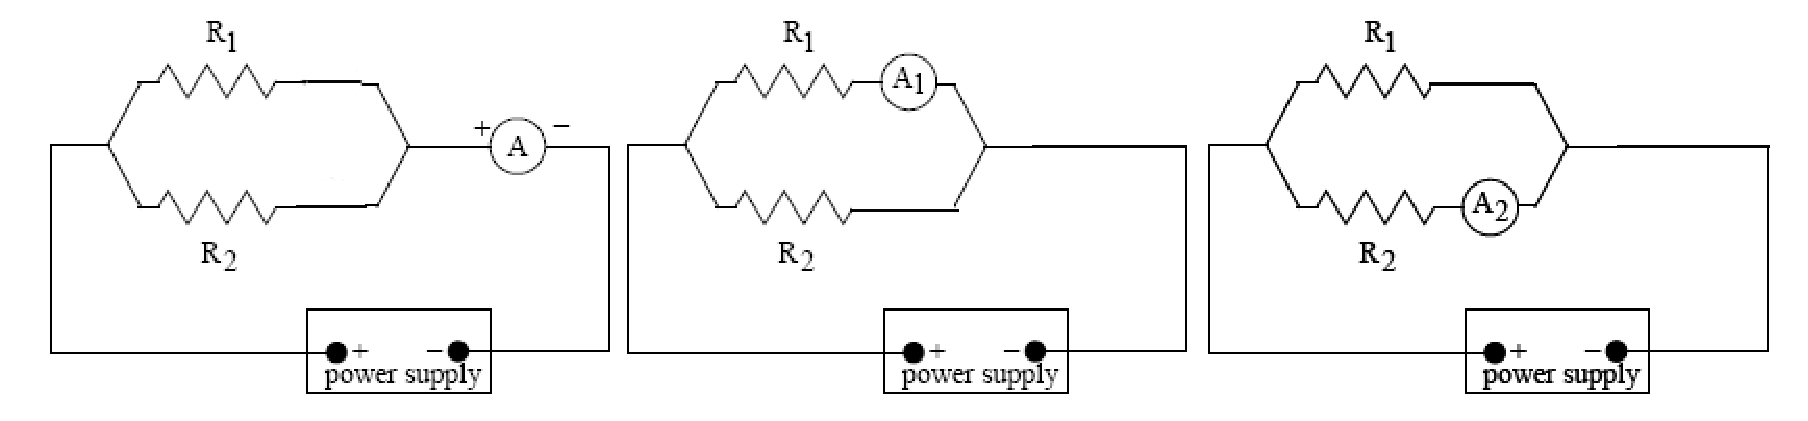
\includegraphics[width=6.0in]{ohms_law_fig_2.eps}
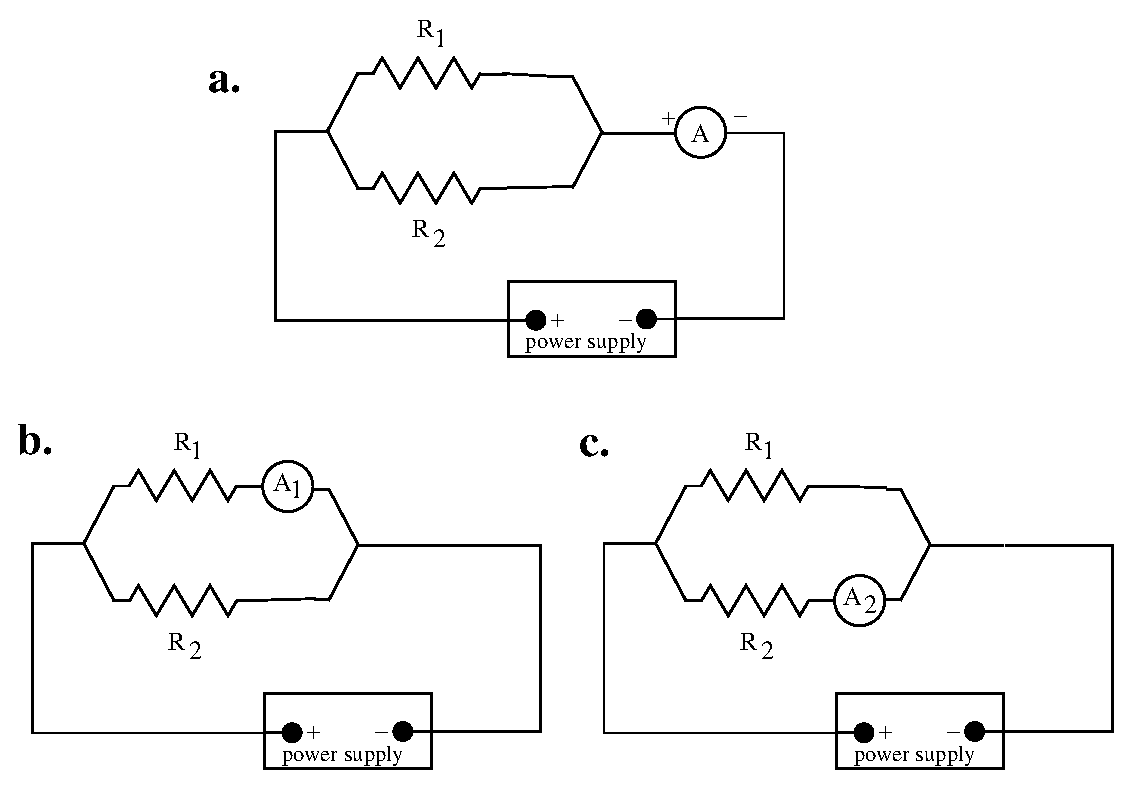
\includegraphics[width=4.6in]{ohms_law/ohms_law_fig_2b.eps}
\end{center}
\vspace{0.3cm}

\begin{itemize}
\item When you are sure the circuit is set up correctly, turn on the power 
supply and turn the coarse voltage control up to about 10 volts. Record the 
total current through the circuit and the voltage across 
the parallel resistance combination. Also measure the voltage across the 
milliammeter (which may be in millivolts). Turn off the power supply.
\vspace{20mm}

\item Connect the milliammeter to the point marked A\( _{1} \) in figure 
\textbf{b} above, without disturbing the rest of the circuit. Turn on the 
 power supply and 
record the current through R\( _{1} \) and the voltage across the parallel 
combination. Turn off the power supply.
\vspace{20mm}

\item Repeat the above measurements for R\( _{2} \), connecting the 
milliammeter at A\( _{2} \) as in figure \textbf{c} above. Turn off the 
power supply.
\vspace{20mm}

%\item Using Ohm's Law, calculate the two resistances of the parallel connection
%and also the total resistance of the circuit. Check with the ohmmeter
%and determine the percent differences.\vspace{30mm}

\item What is the relationship between the total current and the current
in each of the branches of the parallel circuit? (This is an example of 
Kirchhoff's junction rule which is based on conservation of charge.)
\vspace{30mm}

\item Using Ohm's Law and your data above, calculate the resistance of each 
resistor and the total resistance of the circuit.
\vspace{60mm}

\item What is the relationship between the total resistance of the parallel
circuit and the resistance of each of the branches? Using this relationship, 
calculate the total resistance of the circuit from the individual resistances 
you determined above. Does the result agree with what you calculated in the 
previous item? Calculate a percent difference and record it here.


%\item Determine, using Ohm's law, what the voltage was in each branch of
%the parallel circuit. Did it make any difference that you didn't reposition
%the voltmeter during this activity? On the basis of Ohm's law, does
%the result make sense?\vspace{30mm}

%\item Can the total resistance of a series combination ever be less than
%the resistance of the largest resistor? Explain.\vspace{30mm}

%\item Can the total resistance of a parallel combination ever be greater
%than the resistance of the smallest resistor? Explain.\vspace{30mm}
\end{itemize}



\section{Nuclear Decay and Radiocarbon Dating}

Name \rule{2.0in}{0.1pt}\hfill{}Section \rule{1.0in}{0.1pt}\hfill{}Date
\rule{1.0in}{0.1pt}

\textbf{Objective}

To develop an understanding of the use of the radioactive decay of
atomic nuclei to date objects like the Shroud of Turin.

\textbf{Apparatus}

\begin{itemize}

\item Radioactive sources.
\item Radiation counter.
\item Jack.
\item Isotope generator.
\item Surgical gloves, eye protection, and lab coat for handling radioactive liquids.
\item Lead and plastic sheets.

\end{itemize}

\textbf{Introduction}

Atoms can be broken down into light, negatively-charged, electrons,
and a small, dense, positively-charged nucleus. These atomic nuclei
can spontaneously break apart into smaller nuclei in a process called
radioactive decay. By measuring the rate of this decay under the appropriate
circumstances one can develop a {}``clock'' that can be used to
determine how long ago in the past an event occurred. In this laboratory
we will apply this notion to a particular object, the Shroud of Turin
which is purported to be the burial cloth of Jesus Christ.

\textbf{Activity 1: Nuclear Terminology }

Atomic nuclei can be constructed from protons and neutrons. The number
of protons in a nucleus is called the atomic number and is represented
by the letter Z while the number of neutrons is represented by the
letter N. The protons carry a charge of +e while the neutrons are
electrically neutral. The sum of these two quantities is the mass
number A.

{\centering A = N + Z\par}

Protons and neutrons are often referred to as nucleons.

Nuclei are represented using their chemical symbol (determined by
the atomic number) and the mass number. For example, the most common
form of carbon has six protons and six neutrons in its nucleus and
is written as \( ^{12} \)C. If another neutron is added to this nucleus,
then one has an isotope of carbon, \( ^{13} \)C. Isotopes of a chemical element
have the same atomic number(Z), but have a different numbers of neutrons
(N) and a different mass number (A). The difference is reflected in
the value of the superscript on the chemical symbol.

(a) Consider the following list of the number of protons and neutrons
that combine to form a particular nucleus. In the third column enter the chemical
symbol and mass number as shown above (e.g., \( ^{12} \)C). Use the
periodic chart at the end of this unit to determine what to enter in the third
column.

\vspace{0.3cm}
{\centering \begin{tabular}{|c|c|c|}
\hline 
Number of Protons&
Number of Neutrons&
Nucleus\\
\hline
\hline 
7&
8&
\\
\hline 
79&
118&
\\
\hline 
26&
30&
\\
\hline
\end{tabular}\par}
\vspace{0.3cm}

(b) Consider the following list of atomic nuclei. In the second and
third columns enter the number of protons and neutrons in each nucleus.

\vspace{0.3cm}
{\centering \begin{tabular}{|c|c|c|}
\hline 
Nucleus&
Number of Protons&
Number of Neutrons\\
\hline
\hline 
\( ^{4} \)He&
&
\\
\hline 
\( ^{235} \)U&
&
\\
\hline 
\( ^{108} \)Ag&
&
\\
\hline
\end{tabular}\par}
\vspace{0.3cm}

Some isotopes can spontaneously decay into other nuclei.
In many of these decays the number of nucleons is conserved. 
This
means that the number of protons and neutrons added together in the parent nucleus before
the decay must be the same in the final products.
Electric charge
is always conserved.

(c) In the table below a nuclear decay is shown in the first column.
In most cases the original nucleus (often referred to as the parent)
produces two smaller nuclei (called daughters). Only one of the
daughter nuclei is listed. In the adjacent column list the missing
nucleus.
Notice there are two emitted particles that we have not mentioned
before.
The $e^-$ which is an electron and is often called a
beta particle.
It has almost zero mass compared to a nucleon.
The other is $\gamma$ and is called a ``gamma'' particle.
This is photon or a particle of light
or electromagnetic energy.
The gamma has no mass or charge, but does carry energy and momentum.

\vspace{0.3cm}
{\centering \begin{tabular}{|c|c|}
\hline 
~~~~~~~~~~~~~Decay~~~~~~~~~~~~~&
~~~~~~~~Unknown~~~~~~~~\\
\hline
\hline 
\( ^{190} \)Po \( \rightarrow  \) \( ^{4} \)He + ?&
\\
\hline 
\( ^{210} \)Th \( \rightarrow  \) \( ^{4} \)He + ?&
\\
\hline 
\( ^{16} \)Ne \( \rightarrow  \) p + ?&
\\
\hline 
\( ^{90} \)Sr \( \rightarrow  \) \(e^-\) + ?&
\\
\hline 
\( ^{60} \)Co \( \rightarrow  \) \(\gamma\) + ?&
\\
\hline
\end{tabular}\par}
\vspace{0.3cm}

% \textbf{Activity 2: Calibrating the Geiger Counter} 

%Before we proceed we have to understand how to use the device that will detect
%the radiation from radioactive material.
%The device is called a Geiger counter and it will ``count'' the number
%of nuclear particles that pass through it.
%The device consists of a sealed cylinder with a wire
%running down the center and argon gas filling the cylinder.
%The center wire is kept at a large, positive voltage while the walls of the cylinder
%are at zero or negative voltage.
%When an energetic nuclear particle passes through the counter it ionizes the argon
%atoms in the cylinder.
%The electrons are attracted to the center wire and produce a voltage pulse which is
%detected and counted by the electronics. 
%To count the number of particles that pass through the detector accurately
%the voltage of the center wire must be set to produce the same signal regardless of the energy
%of the particle passing through the Geiger tube.
%To find this ``plateau'' voltage follow the procedure below.

%(a) Make sure the Geiger counter is plugged into the computer interface and into the power
%supply. If not, consult your instructor.

%(b) There will be a radioactive source at each station for calibrating the Geiger counter.
%The window on the end of the cylinder is very fragile so avoid touching it at all costs.
%Place the radioactive source on the square palette and slip it into one of the slots
%underneath the Geiger counter.

%(c) Start the {\it Geiger Counter Calibration} application. You will see a panel with
%a bunch of options on it.
%Click on Setup and set the ``Count Time Period'' to something like 0.5-1.0 minutes.
%Click ``Done'' when you are finished.

%(d) Turn the Geiger counter on using the switch on the barrel of the detector.
%(e) Now click ``Record'' on the {\it Geiger Counter Calibration} application.
%The device will count the number of nuclear particles striking the Geiger counter
%for the time period you set above.
%This count will show in the panel at the bottom, right-hand portion of the
%window.
%The count rate should be
%about zero.

%(f) Slowly turn up the voltage.
%This can be done by clicking on ``Voltage'' and entering a value in the pop-up window.
%Increase this voltage in steps no large than 100 volts 
%until the Geiger Counter starts counting at an appreciable
%rate. 
%This is called the threshold voltage. record this value in the table below.

%(g) Now start increasing the voltage on the Geiger counter in steps of 25 volts
%and recording the number of counts per minute in your chosen time period.
%Make sure you divide the number of counts you record by the length of the time
%period.
%Use the space below to record your results.
%You should see the count rate increase rapidly at first as you raise the
%voltage.
%Eventually, the count rate will level off and be constant as the voltage is
%increased. When this levelling off occurs you have found the plateau.
%See the figure below.
%You will set the voltage on the Geiger counter in the center of this plateau
%in the remaining 
%activities.

%\vspace{0.3cm}
%{\centering \resizebox*{0.4\textwidth}{!}{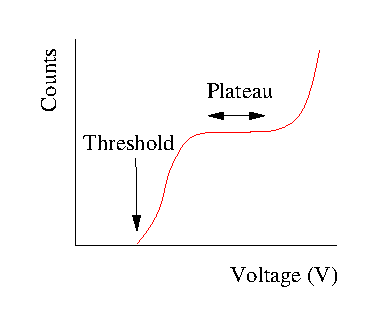
\includegraphics{radiocarbon_dating/geiger1.eps}} \par}
%\vspace{0.3cm}

%(h) Make a plot of counts per minute versus voltage and attach it to your unit.
%Check with your instructor that it looks acceptable.

%\vspace{3.0in}

\textbf{Activity 2: The Properties of Radiation}

An essential attribute of radiation is its ability to penetrate
matter.
Here we will study how three different types of radiation (alpha, beta,
and gamma radiation) penetrate matter. We will do this by using a radiation counter
 and samples of three nuclei.
The heart of the radiation counter is a gas-filled cylinder with a wire at
high voltage running down its center.
This cylinder is called a Geiger-Muller or G-M tube.
Sub-atomic particles flying through the counter ionize atoms in the gas which are 
collected at the center wire producing a voltage pulse that can be measured.
NOTE: Before going any further read the appendix on nuclear safety.

(a) Compare the figure below with your setup. Familiarize yourself with the
different components. DO NOT TOUCH THE FACE OF THE DETECTOR INSIDE
THE SNOUT UNDER ANY CIRCUMSTANCES.

\vspace{0.3cm}
{\centering \resizebox*{0.5\textwidth}{!}{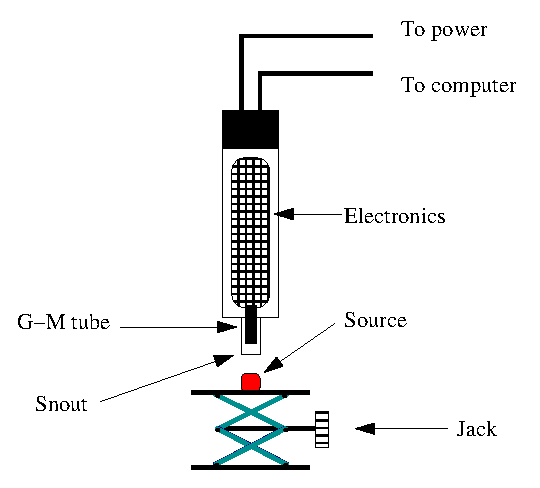
\includegraphics{radiocarbon_dating/rad_counter.eps}} \par}
{\centering Figure 1. Schematic drawing of radiation counter and setup. \par}
\vspace{0.3cm}

(b) Carefully remove the red, plastic cover on the snout of the radiation counter.
DO NOT TOUCH THE FACE OF THE DETECTOR UNDER ANY CIRCUMSTANCES. This would likely
break the window and destroy the counter.

(c) Obtain a set of radioactive sources from your instructor.
Pick one of the sources, place it on the jack, and position the source about 1 cm below
the snout of the radiation counter.
Plug the power cord into a standard electric outlet and make sure the data cable is plugged
into digital channel 1 on the {\it DataStudio} 750 interface.
You should see the power light come on near the base of the counter (which is actually at the
top).
Another light near the snout of the counter blinks whenever a particle
is detected.
If you don't see either light, consult your instructor.

(d) Open the {\it Radiation Counter} activity in the {\bf 132 Workshop} menu and click
the {\bf Start} button on the {\it DataStudio} interface.
Nothing will seem to be happening, but after 30 seconds (watch the clock at the top
of the {\it DataStudio} interface) the number of radioactive decays detected by the 
radiation counter will appear.
Record this result in the appropriate place in the table below.

(e) Now carefully place a piece of plastic on top of the source and run the
counter for another 30 seconds. Record the result below.

(f) Remove the plastic and place a small sheet of lead on top of the source.
Run the counter and record the result.

(g) Repeat steps d-f for the other two radioactive sources.


\vspace{0.3cm}
{\centering \begin{tabular}{|c|c|c|c|}
\hline 
Radiation&
~~~Air~~~~&
~~Plastic~&
~~~Lead~~~\\
\hline
\hline 
\( \gamma \)&
&
&
\\
\hline 
\( \beta \)&
&
&
\\
\hline 
\( \alpha \)&
&
&
\\
\hline
\end{tabular}\par}
\vspace{0.3cm}

(h) Which type of radiation is most penetrating? Why?
\vspace{15mm}

(i) Which type of radiation is least penetrating? Why?
\vspace{15mm}

(j) What material provides the best shielding of radioactivity? Why?
\vspace{15mm}

\textbf{Activity 3: Background Radiation}

(a) Return the radioactive sources to the instructor's table.

(b) With no radioactive sources nearby, make several runs with the radiation counter.
The counts you observe in the detector are due to cosmic rays, radioactive decay
in the building materials surrounding you, and even your own body.
Record the counts and calculate the average and standard deviation of this background
radiation.
\vspace{15mm}

\vspace{1.0in}


\textbf{Activity 4: Nuclear Decay }

To understand the ``clock'' we will use to date the Shroud of Turin we will investigate
how the clock ``ticks''.
In this activity you will use a sample of radioactive material and a nuclear to 
detector to measure the behavior of the material as a function of time.
We will then build a mathematical model of the time dependence of nuclear decay.
We will apply this model to analyze the results of $\rm ^{14}C$ measurements on
the Shroud.

To obtain the radioactive material we will use a procedure known as
``milking the cow''.
We start with a liquid that contains the radioactive isotope $\rm ^{137}Cs$ or
cesium-137.
This isotope decays very slowly; it would take about 30 years for half of a sample
to decay (a bit long for an introductory physics experiment).
However, when $\rm ^{137}Cs$ does decay it usually does so in the following way.

{\centering \( \rm ^{137}Cs \rightarrow e^- + ^{137}Ba(0.662) \) \par}

Notice the additional number ``0.662'' beside the Ba-137. This number means there
is still some energy (0.662 million electron-volts or MeV)
stored in the Ba-137 nucleus and it has not yet reached
its lowest-energy or ground state.
This ``excited'' state of Ba-137 then emits a high-energy photon or gamma ray to 
reach the stable ground state of $\rm {^{137}Ba}$. A diagram of the
process is below. 

\vspace{0.3cm}
{\centering \resizebox*{0.5\textwidth}{!}{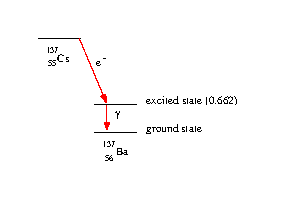
\includegraphics{radiocarbon_dating/Cs-137_decay.eps}} \par}
{\centering Figure 2. Decay scheme of cesium-137. \par}
\vspace{0.3cm}

This intermediate state (labeled ``0.662'') decays quickly to the ground state and
it is the one we will study.

We will prepare a sample of Ba-137 in its excited, 0.662-MeV state 
by starting with a Cs-137 ``generator''.
The Cs-137 produces
Ba-137 at a steady rate. We remove the Ba-137 from the ``generator''
by passing a hydrochloric-acid-saline solution through the generator
(your instructor will do this). This is called eluting which means separate by
washing. The generator is commonly referred to as the ``cow''
and the Ba-137 is ``milked'' from the cow.
The Ba-137 is eluted from the generator and can then be used to study its
decay.


(a) First, make a prediction of the count rate as a function of time.
Sketch your prediction in the space below.

\vspace{1.5in}

(b) What is the mathematical form of your prediction? Why did you choose it?

\vspace{1.5in}

(c) Open the {\it Nuclear Decay} application in the {\bf 132 Workshop} menu. 
When you click {\bf Start}
it will plot the count rate in intervals of 10 seconds.
Get the radioactive sources from your instructor and
try this out with one of them
to make sure you know how to use the hardware and software.
Return the sources to your instructor when you are finished with this test.

(d) Read the rest of this procedure carefully. 
If you have to redo the procedure it may take a long time for the ``generator'' to
produce enough Ba-137 for you to use.

(e) You have a small, metal disk called a planchette that sits on the 
jack which will be positioned close to the snout of the radiation counter.
This will hold the radioactive material.
Put the empty planchette in place and do a ``dry run''.

(f) One team member should be responsible for positioning the planchette.
That person should put on the surgical gloves, eye protection, and a lab coat.
The other team member can run the data acquisition.

(g) When you are ready, alert the instructor. He or she will come over and place 
a few drops of the eluate containing the Ba-137 on the planchette.
Immediately place this under the Geiger counter and
click {\bf Start} on the {\it DataStudio} interface.

{\bf Caution:} Care should be taken in handling the sample.
If any portion of the sample touches your skin immediately wash off in the sink.

(h) Let the data acquisition run for about fifteen minutes or so and then click {\bf Stop}.
Dispose of the planchette according to the guidance from the instructor.

(i) Make a plot of your results using the data in the {\it Counts versus Time Table}. 
Notice that if you 
click on the title of the table, all of the
data will be selected. You can then paste the data into {\it Excel}.
Make sure you subtract the background radiation from your results.

(j) Make a fit to your data. What is the best choice of function for fitting 
your data? How did you make your choice?
Attach a copy of your plot with the fit to this unit.
Record the fit equation below.
Do NOT close your spreadsheet. We may use it later.

\vspace{0.5in}

\textbf{Activity 5: Analyzing Nuclear Decay }

Observation of a sample of radioactive material reveals that the decay
of the atomic nuclei in the sample is determined by statistical processes.
In other words, the number of nuclei N\( _{nuc} \) that decay per
unit time is proportional to the number of nuclei in the sample.

\[
\frac{dN_{nuc}}{dt}\propto N_{nuc}\]


This expression can be turned into an equality by inserting a constant
of proportionality \( \lambda  \) so

\[
\frac{dN_{nuc}}{dt}=-\lambda N_{nuc}\]


where the minus sign is needed because the number of nuclei N\( _{nuc} \)
decreases with time. The decay constant \( \lambda  \) is a characteristic
of each atomic nucleus. 

(a) In the previous activity, you used a particular function to fit 
your data.
Try to prove that you made the right choice by taking derivatives and
seeing if they will satisfy the original differential equation above.
Did it work?
\vspace{30mm}

(b) It is claimed the solution of the differential equation above
describing nuclear decay is the following expression.

\[
N_{nuc}(t)=N_{0}e^{-\lambda t}\]


Prove this statement by taking the derivative of N\( _{nuc} \)(t)
and showing it satisfies the original differential equation. Make
a sketch of the function and describe it in words.
How did your fit function do?
\vspace{40mm}

(c) The decay of atomic nuclei is often characterized by a quantity
known as the half-life \( \tau  \). The half-life is the period of
time for one-half of the original sample to disappear via radioactive
decay. This statement can be expressed mathematically in the following
way.

\[
N_{nuc}(t=\tau )=\frac{N_{0}}{2}\]


Starting with the above expression show that the decay constant \( \lambda  \)
and the half-life are related by the following equation.

\[
\tau =\frac{\ln 2}{\lambda }\]


\vspace{2in}

(d) Now return to the results of your experiment.
Does your count rate fall off exponentially?
Did you fit your data with an exponential? If not,
go back and do so.
Record the decay constant $\lambda$.
\vspace{0.75in}

(e) What is the half-life of Ba-137? Compare this with the accepted value of 2.552 minutes.
\vspace{1.5in}

(f) Consider the following example as a warm-up. A sample of the isotope of iodine
\( ^{131} \)I has an initial decay rate of 1.8 x 10\( ^{5} \) decays/s.
This isotope has a half-life of 8.04 days. It is shipped to a medical
diagnostic laboratory where it will be used as a radioactive tracer.
When the shipment arrives at the lab the decay rate has fallen to
1.4 x 10\( ^{5} \) decays/s. How long did it take for the shipment
to reach the laboratory?
\vspace{2in}


\textbf{Activity 6: Dating the Shroud of Turin }

The previous example shows how one can use the measured decay rate
of an atomic nucleus as a {}``clock'' to determine the passage of
time. The same concept is used in radiocarbon dating. Carbon on the
planet Earth consists largely of three isotopes with A = 12, 13, and
14. The most common form is \( ^{12} \)C and only a very small fraction
of the carbon is \( ^{14} \)C. However, \( ^{14} \)C decays via 

{\centering \( ^{14} \)C \( \rightarrow  \) \( ^{14} \)N + \( \beta ^{-} \)
+ \( \overline{\nu } \)\par}

where \( \beta ^{-} \) is an electron and \( \overline{\nu } \)
is a particle known as a neutrino. Notice this decay does NOT preserve
the number of protons and neutrons in the original nucleus. The ratio
R of \( ^{14} \)C to \( ^{12} \)C on the Earth is 1.30 x 10\( ^{-12} \)
and is roughly constant despite the fact that the \( ^{14} \)C constantly
disappears. The ratio is constant because the supply of \( ^{14} \)C
in the atmosphere is replenished by the reaction of cosmic rays from
outer space with the nitrogen in the upper atmosphere.

Living organisms contain large quantities of carbon and are constantly
exchanging carbon with their surroundings. They contain the same proportion
of \( ^{14} \)C to \( ^{12} \)C as observed in the atmosphere. However,
this proportion begins to change after the organism dies. The \( ^{12} \)C
remains in the dead body, but the \( ^{14} \)C turns into gaseous
\( ^{14} \)N (see decay above) and leaves the body. Hence, the proportion
of \( ^{14} \)C decreases with time, and one has a {}``clock''
that can be used to determine when an organism died. 

The Shroud of Turin is a piece of cloth that bears the image of a
man who appears to have been crucified. It was first displayed in
France in the fourteenth century and has been kept at the Royal Chapel
of Turin Cathedral in a special shrine since 1694. Many believe the
image on the Shroud is of Christ and the cloth is his burial wrap.
In 1989, three laboratories in Arizona in the USA, Oxford in the UK,
and Zurich in Switzerland used advanced methods of radiocarbon dating
in an attempt to determine the age of the Shroud{[}1{]}. The Shroud
is woven of cloth made from plants. Like a living organism that has
died, the \( ^{14} \)C in the Shroud began to gradually disappear
after the plants used to make it were harvested.

(a) The half-life of \( ^{14} \)C is 5730 years. What is the decay
constant \( \lambda  \)?
\vspace{25mm}

\newpage

(b) The three laboratories obtained the following results for the
ratio R of \( ^{14} \)C to \( ^{12} \)C. The ratio of \( ^{14} \)C
to \( ^{12} \)C in the atmosphere is R\( _{i} \) = 1.30 x 10\( ^{-12} \).
What is the implied age of the Shroud for each measurement? Use the
space below for your calculations and enter the results in the table. 

\vspace{0.3cm}
{\centering \begin{tabular}{|c|c|c|}
\hline 
~~~~~Laboratory~~~~~&
~~~~~~~~R\( _{f} \)~~~~~~~~&
~~~~~Age (years)~~~~~\\
\hline
\hline 
Arizona&
1.20 x 10\( ^{-12} \)&
\\
\hline 
Oxford&
1.18 x 10\( ^{-12} \)&
\\
\hline 
Zurich&
1.19 x 10\( ^{-12} \)&
\\
\hline
\end{tabular}\par}
\vspace{0.3cm}

\vspace{5in}
(c) What is the average age of the Shroud? 
\vspace{1in}

(d) The typical uncertainty in these measurements is a standard deviation
of \( \pm  \)40 years. Are the results of the three laboratories
consistent? 
\vspace{1in}

\vspace{15mm}
(e) Is the age of the Shroud consistent with it being the burial wrap
of Christ? 
\vspace{1in}

(f) Are there any reasons to doubt these results?
\vspace{1in}

\textbf{Homework} 

\begin{enumerate}
\item The half-life of a particular radioactive isotope is 6.5 h. If there
are initially 48 x 10\( ^{19} \) atoms of this isotope, how many
atoms of this isotope remain after 26 h? 
\item A radioactive isotope of mercury, \( ^{197} \)Hg, decays into gold,
\( ^{197} \)Au, with a disintegration constant of 0.0108 h\( ^{-1} \).
(a) What is its half-life? (b) What fraction of the original amount
will remain after three half-lives? (c) What fraction will remain
after 10.0 days?
\item The radionuclide \( ^{64} \)Cu has a half-life of 12.7 h. How much
of an initially pure, 5.50-g sample of \( ^{64} \)Cu will decay during
the 2.0-h period beginning 14.0 h later? 
\end{enumerate}

\textbf{The Periodic Chart} 

\begin{center}
%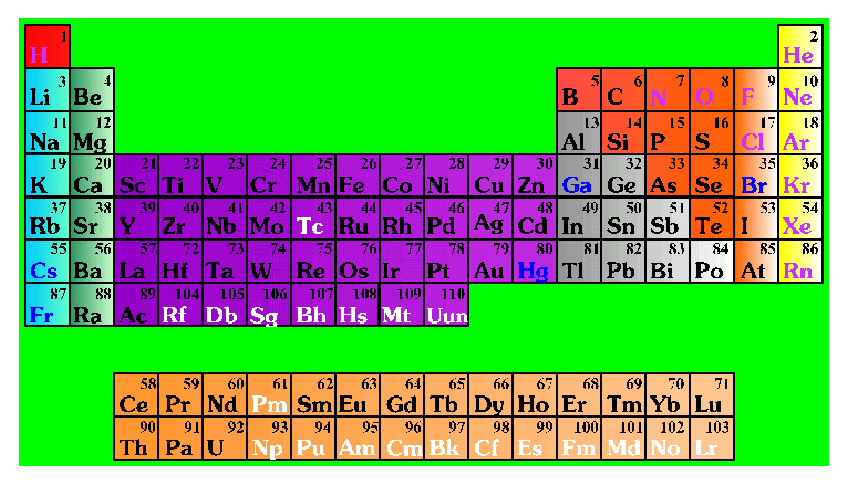
\includegraphics{radiocarbon_dating/pertable2.eps}
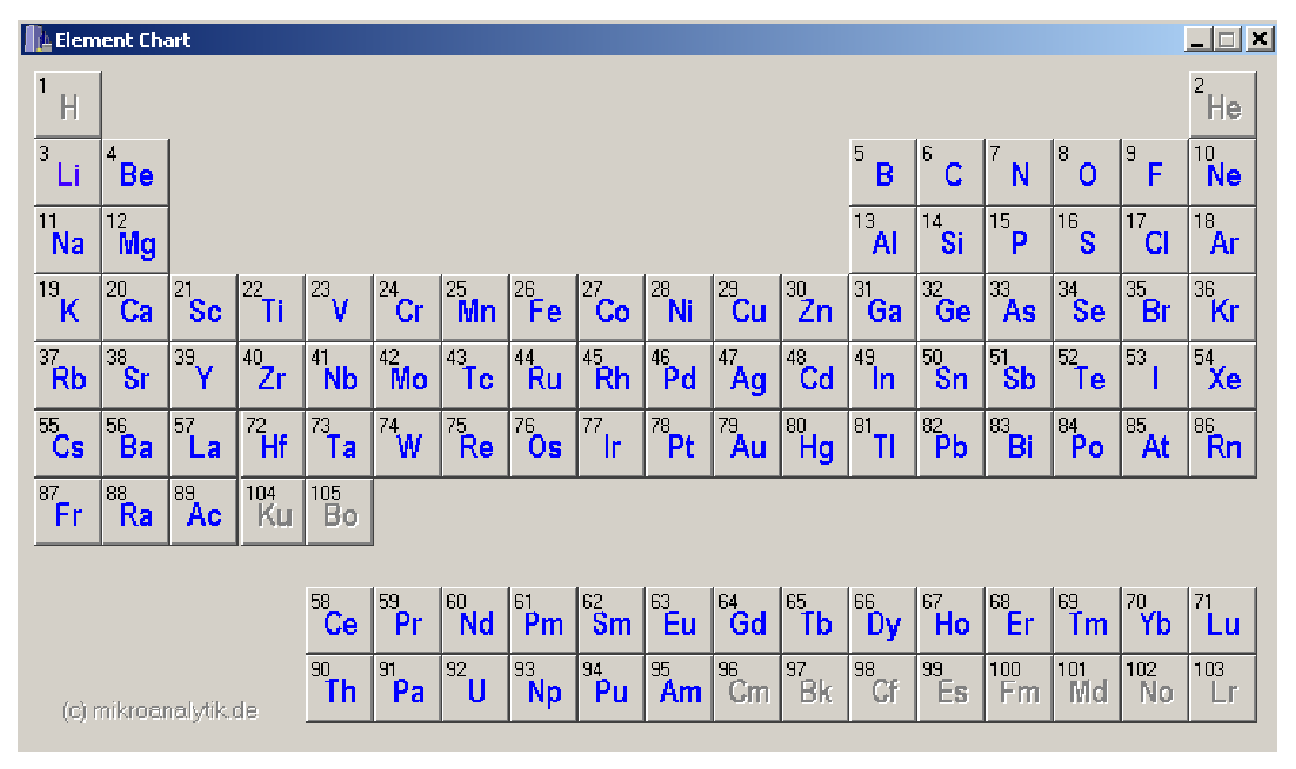
\includegraphics[width=5.5in]{radiocarbon_dating/pertable3.eps}
\end{center}

\textbf{References}

\begin{enumerate}
\item P.E.Damon, D.J.Donahue, B.H.Gore, A.L.Hathaway, A.J.T.Jull, T.W.Linick,
P.J.Sercel, L.J.Toolin, C.R.Bronk, E.T.Hall, R.E.M.Hedges, R.Housley,
I.A.Law, C.Perry, G.Bonani, S.Trumbore, W.Woelfli, J.C.Ambers, S.G.E.Bowman,
M.N.Leese, and M.S.Tite, \emph{Nature}, Vol. \textbf{337}, No. 16,
P. 611-615.\end{enumerate}


%--------------------------------------------
\appendix
\setcounter{section}{4} %set this counter to number MINUS ONE corresponding to desired appendix letter. (4 for `E', etc.)
%Put include statements for supplementary appendices below here.
                                                 
\section{Nuclear Safety}

All of the radioactive sources we will use in class are very low-level
isotopes referred to as ``license-free'' sources.
The following guidelines should be followed for handling radioactive
materials in the classroom.

%test comment by Matt
\begin{enumerate}

\item Eating, drinking, and application of cosmetics in the 
laboratory are not permitted.

\item Pipetting by mouth is never permitted. Use suction devices
such as pipette filters.

\item Gloves and lab coats should be worn when working with all liquid
isotopes.

\item Before leaving the lab, wash your hands thoroughly and check for
possible contamination with a survey instrument.

\item All radioactive liquid wastes are to be poured into the liquid
waste container, NEVER into a sink.

\item Report all spills, wounds, or other emergencies to your instructor.

\item Maintain good housekeeping at all times in the lab.

\item Store radioactive material only in the designated storage area. Do not
remove sources from the lab.

\end{enumerate}


\end{document}
